\documentclass[a4]{article}
\usepackage{graphicx}
%\def\C++{{\rm C\kern-.05em\raise.3ex\hbox{\footnotesize ++}}}
%\def\underscore{\leavevmode\kern.04em\vbox{\hrule width 0.4em height 0.3pt}}
\setlength{\parindent}{0pt}                                                                              
%\setlength{\textwidth}{6.5in}
%\setlength{\oddsidemargin}{0.0in}                                                                                  
\usepackage{hyperref}

\title{Marking up differences between latex files with {\em latexdiff}}
\author{F.J. Tilmann\thanks{tilmann@gfz-potsdam.de}}
\date{\today}

\begin{document}
\maketitle

\section*{Preamble}

{\em latexdiff} is a Perl script, which compares two
latex files and marks up significant differences between them.  Various options are available for visual markup using standard
latex packages such as {\em color.sty}. Changes not directly affecting visible
text, for example in formatting  commands, are still marked in the
latex source.

A rudimentary revision facility is provided by another Perl script,
{\em latexrevise}, which  accepts or rejects all changes.  Manual editing
of the difference file can be used to override this default behaviour
and accept or reject selected changes only.  

There is no explicit support for annotations as these are trivial to implement.
For example, I include the following command definition in the preamble
\begin{verbatim}
\newcommand{\remark}[1]{{ \bf [ \footnotesize #1 ]}}
\end{verbatim}
and mark up annotations as follows 
\begin{verbatim}
... The roadrunner is the fastest running bird  \remark{Check this 
again with a zoologist!}. The most famous roadrunner ...
\end{verbatim}
Alternatively, instead of a command like \verb#\remark# in the example just given, an
equivalent annotation environment could be defined.
{\em latexrevise} can  remove such comments or
environments from the text body.

%It is planned that the revision capabilities of this system will be
%further expanded, dependent on the amount of feedback received.

On the following pages you find  the {\em man} pages for {\em
  latexdiff} and {\em latexrevise} and a simple example.

\include{latexdiff}
\setcounter{section}{0}

\include{latexrevise}
\setcounter{section}{0}

\include{latexdiff-vc}
\setcounter{section}{0}

\section*{A simple example}

We start with a draft text, \verb|example-draft.tex|, listed here in
full but also included in the distribution (except that the ``verbatim'' environment had
to be renamed to ``Verbatim'' for the listing).

{\scriptsize
\begin{verbatim}
\documentclass[12pt,a4paper]{article}

\setlength{\topmargin}{-0.2in}
\setlength{\textheight}{9.5in}
\setlength{\oddsidemargin}{0.0in}

\setlength{\textwidth}{6.5in}

\title{latexdiff Example - Draft version}
\author{F Tilmann}

\begin{document}
\maketitle

\section*{Introduction}

This is an extremely simple document that showcases some of latexdiff features.
Type
\begin{Verbatim}
latexdiff -t UNDERLINE example-draft.tex example-rev.tex > example-diff.tex
\end{Verbatim}
to create the difference file.  You can inspect this file directly. Then run either 
\begin{Verbatim}
pdflatex example-diff.tex
xpdf example-diff.pdf
\end{Verbatim}
or
\begin{Verbatim}
latex example-diff.tex
dvips -o example-diff.ps example-diff.dvi
gv example-diff.ps
\end{Verbatim}
to display the markup. Of course, instead of \verb|xpdf| you can use 
\verb|okular, evince, acroread| or any other pdf or postscript viewer.

\section*{Another section title}

A paragraph with a line only in the draft document.  More things 
could be said were it not for the constraints of time and space.

More things could be said were it not for the constraints of time and space.

And here is a tipo. 

Here is a table:

\begin{tabular}{ll}
Name & Description \\
\hline
Gandalf & Grey \\
Saruman & White
\end{tabular}

And sometimes a whole paragraph gets completely rewritten. In this
case latexdiff marks up the whole paragraph even if some words in it
are identical.
No change, no markup!
\end{document}
\end{verbatim}
}

We can now edit
this text as we would do with any other latex file to create
a new revision of the text, \verb|example-rev.tex|.  We should run
\begin{verbatim}
latex example-rev.tex
\end{verbatim}
and look at the resulting \verb|.dvi| file to make sure that all
changes are valid.  An example revision is listed here:

{\scriptsize
\begin{verbatim}
\documentclass[12pt,a4paper]{article}

\setlength{\topmargin}{-0.2in}
\setlength{\textheight}{9.5in}
\setlength{\oddsidemargin}{0.0in}

\setlength{\textwidth}{6in}

\title{latexdiff Example - Revised version}
\author{F Tilmann}
% Note how in the preamble visual markup is never used (even
% if some preamble might eventually end up as visible text.)

\begin{document}
\maketitle

\section*{Introduction}

This is an extremely simple document that showcases some of the latexdiff features.
Type
\begin{Verbatim}
latexdiff -t UNDERLINE example-draft.tex example-rev.tex > example-diff.tex
\end{Verbatim}
to create the difference file.  You can inspect this file directly. Then run either 
\begin{Verbatim}
pdflatex example-diff.tex
xpdf example-diff.pdf
\end{Verbatim}
or
\begin{Verbatim}
latex example-diff.tex
dvips -o example-diff.ps example-diff.dvi
gv example-diff.ps
\end{Verbatim}
to display the markup.

\section*{Yet another section title}

 More things could be said were it not for the constraints of time and space.

A paragraph with a line only in the revised document.  
More things could be said were it not for the constraints of time and space.

And here is a typo. 

Here is a table:

\begin{tabular}{ll}
Name & Description \\
\hline
Gandalf & White \\
Saruman & Evil
\end{tabular}

And now for something completely different, with not a paragraph in sight.
No change, 
no markup!
\end{document}
\end{verbatim}
}

To compare both revisions, type
\begin{verbatim}
latexdiff -t UNDERLINE example-draft.tex example-rev.tex > example-diff.tex
\end{verbatim}
This results in the following difference file (a few newlines have been 
added in this listing for legibility reasons):
{\scriptsize
\begin{verbatim}
\documentclass[12pt,a4paper]{article}

\setlength{\topmargin}{-0.2in}
\setlength{\textheight}{9.5in}
\setlength{\oddsidemargin}{0.0in}

%DIF 7c7
%DIF < \setlength{\textwidth}{6.5in}
%DIF -------
\setlength{\textwidth}{6in} %DIF > 
%DIF -------

%DIF 9c9
%DIF < \title{latexdiff Example - Draft version}
%DIF -------
\title{latexdiff Example - Revised version} %DIF > 
%DIF -------
\author{F Tilmann}
% Note how in the preamble visual markup is never used (even %DIF > 
% if some preamble might eventually end up as visible text.) %DIF > 
%DIF PREAMBLE EXTENSION ADDED BY LATEXDIFF
%DIF UNDERLINE PREAMBLE %DIF PREAMBLE
\RequirePackage[normalem]{ulem} %DIF PREAMBLE
\RequirePackage{color} %DIF PREAMBLE
\providecommand{\DIFadd}[1]{{\color{blue}\uline{#1}}} %DIF PREAMBLE
\providecommand{\DIFdel}[1]{{\color{red}\sout{#1}}}                      %DIF PREAMBLE
%DIF SAFE PREAMBLE %DIF PREAMBLE
\providecommand{\DIFaddbegin}{} %DIF PREAMBLE
\providecommand{\DIFaddend}{} %DIF PREAMBLE
\providecommand{\DIFdelbegin}{} %DIF PREAMBLE
\providecommand{\DIFdelend}{} %DIF PREAMBLE
%DIF FLOATSAFE PREAMBLE %DIF PREAMBLE
\providecommand{\DIFaddFL}[1]{\DIFadd{#1}} %DIF PREAMBLE
\providecommand{\DIFdelFL}[1]{\DIFdel{#1}} %DIF PREAMBLE
\providecommand{\DIFaddbeginFL}{} %DIF PREAMBLE
\providecommand{\DIFaddendFL}{} %DIF PREAMBLE
\providecommand{\DIFdelbeginFL}{} %DIF PREAMBLE
\providecommand{\DIFdelendFL}{} %DIF PREAMBLE
%DIF END PREAMBLE EXTENSION ADDED BY LATEXDIFF

\begin{document}
\maketitle

\section*{Introduction}

This is an extremely simple document that showcases some of latexdiff features.
Type
\begin{Verbatim}
latexdiff -t UNDERLINE example-draft.tex example-rev.tex > example-diff.tex
\end{Verbatim}
to create the difference file.  You can inspect this file directly. Then run either 
\begin{Verbatim}
pdflatex example-diff.tex
xpdf example-diff.pdf
\end{Verbatim}
or
\begin{Verbatim}
latex example-diff.tex
dvips -o example-diff.ps example-diff.dvi
gv example-diff.ps
\end{Verbatim}
to display the markup.

\section*{\DIFaddbegin \DIFadd{Yet another }\DIFaddend \DIFdelbegin 
\DIFdel{Another }\DIFdelend section title}

 \DIFdelbegin \DIFdel{A paragraph with a line only in the draft
   document.  }\DIFdelend More things could
 be said were it not for the constraints of time and space.

\DIFaddbegin \DIFadd{A paragraph with a line only in the revised
  document.  }\DIFaddend More things could be said 
were it not for the constraints of time and space.

And here is a \DIFaddbegin \DIFadd{typo}\DIFaddend \DIFdelbegin 
\DIFdel{tipo}\DIFdelend . 

Here is a table:

\begin{tabular}{ll}
Name & Description \\
\hline
Gandalf & \DIFaddbegin \DIFadd{White }\DIFaddend \DIFdelbegin 
\DIFdel{Grey }\DIFdelend \\
Saruman & \DIFaddbegin \DIFadd{Evil
}\DIFaddend \DIFdelbegin \DIFdel{White
}\DIFdelend \end{tabular}

And \DIFaddbegin \DIFadd{now for something completely different, with not
 a paragraph in sight}\DIFaddend \DIFdelbegin \DIFdel{sometimes a whole
 paragraph gets completely rewritten. In this
case latexdiff marks up the whole paragraph even if some words in it
are identical}\DIFdelend .
No change, 
no markup!
\end{document}
\end{verbatim}
}
Type 
\begin{verbatim}
pdflatex example-diff.tex
xpdf example-diff.pdf
\end{verbatim}
to make the markup visible. This is what it looks like:

\vspace{1cm}
\framebox[\textwidth]{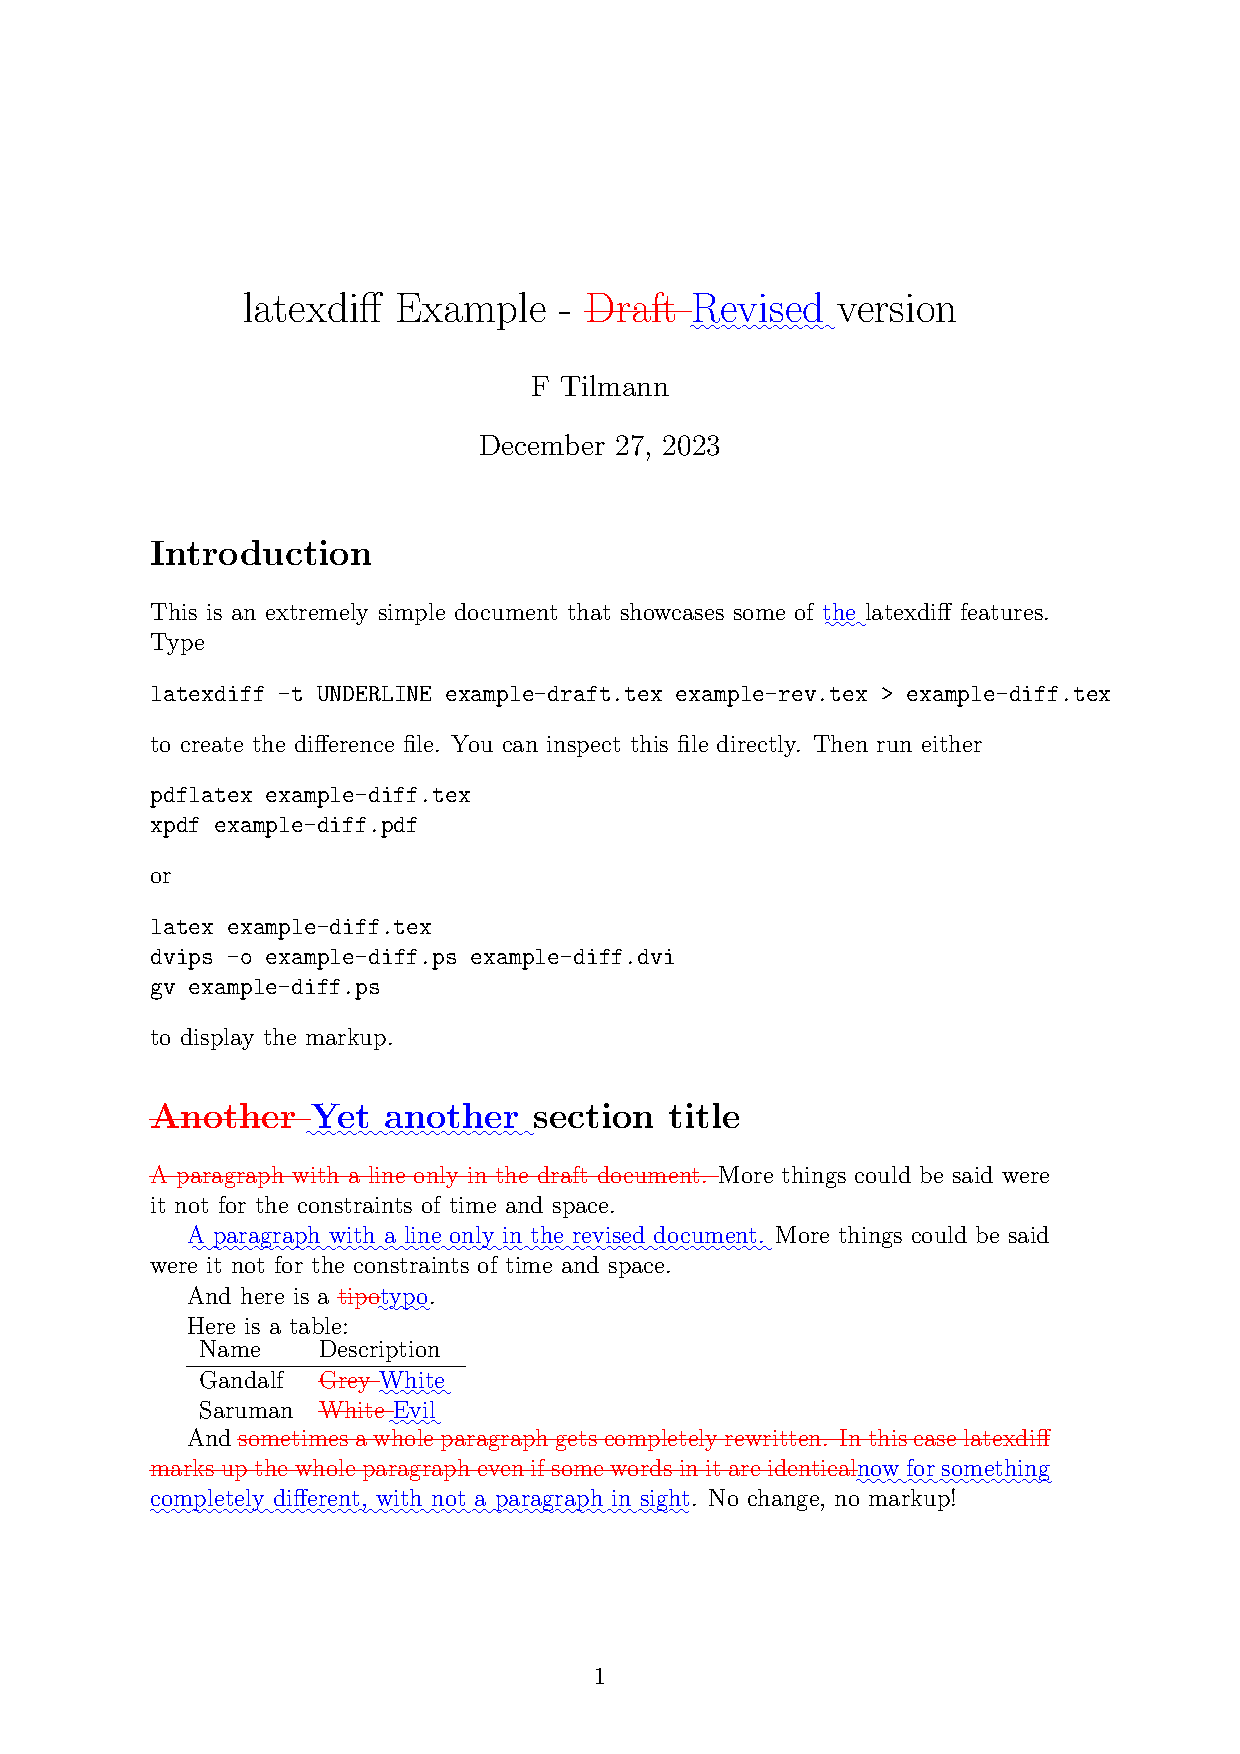
\includegraphics[width=\textwidth]{example-diff}}
\vspace{1cm}

If you approve of all the changes in the revision, just continue with 
\verb|example-rev.tex| for the next revision.  If you like to adopt
most but not all changes you can use \verb|latexrevise| in the
following manner.  Simply edit \verb|example-diff.tex| to remove the \verb|\DIFdelbegin| and
\verb|\DIFdelend| tags around the text you would like to keep and
simply remove the text between  \verb|\DIFaddbegin| and
\verb|\DIFaddend| tags, if you do not wish to keep them.  Say you are happy with all proposed changes for the
example above except in
the last paragraph where you prefer the original draft.  You have
to change

{\scriptsize
\begin{verbatim}
...
And \DIFaddbegin \DIFadd{now for something completely different, with not
 a paragraph in sight}\DIFaddend \DIFdelbegin \DIFdel{sometimes a whole
 paragraph gets completely rewritten. In this
case latexdiff marks up the whole paragraph even if some words in it
are identical}\DIFdelend .
...
\end{verbatim}
}
into 
{\scriptsize
\begin{verbatim}
...
And \DIFdel{sometimes a whole
 paragraph gets completely rewritten. In this
case latexdiff marks up the whole paragraph even if some words in it
are identical}.
...
\end{verbatim}
}
and run 
\begin{verbatim}
latexrevise -a example-diff.tex > example-final.tex
\end{verbatim}
\verb|example-final.tex| is then almost identical to 
\verb|example-rev.tex| except for the last paragraph.

\section*{External tools}
The following is an incomplete list of wrappers written by others providing some added functionality. These are not included with the distribution but need to be downloaded and installed separately.

\begin{description}
 \item[latexdiffcite] (Author: Christer van der Meeren)  is a wrapper around latexdiff to make citations diff properly. It works by expanding \verb|\cite| type commands using the bbl or bib file, such that citations are treated just like normal text rather than as atomic in the plain latexdiff. \\
\url{https://latexdiffcite.readthedocs.org}
\item[git-latexdiff] (lead author: Matthieu Moy) is a wrapper (bash script) around latexdiff that allows using it to diff two revisions of a \LaTeX file under git revision control Similar functionality is provided by \verb|latexdiff-vc --git| with \verb|--flatten| option included with this distribution but git-latexdiff allows more fine-grained control on various aspects. (Not to be confused with latexdiff-git, which is normally installed as a soft link to latexdiff-vc) \\
\url{https://gitlab.com/git-latexdiff/git-latexdiff}

\end{description}

\end{document}
